\documentclass[a4paper,12pt]{report}
\usepackage{graphicx}
\usepackage[utf8]{inputenc}
\usepackage{url}
\usepackage{pdfpages}
\usepackage[italian]{babel}
\usepackage[italian]{cleveref}

\title{Elaborato per il corso Basi di Dati\\ \small Progetto di una base di dati per la gestione di un sito di e-Commerce}

\author{
    Studente: Emma Leonardi\\
    Email: \url{emma.leonardi2@studio.unibo.it}\\
    Matricola: 0000971438\\
    A.A. 2021/2022
    }
\date{}
\begin{document}

\maketitle
\tableofcontents

\chapter{Analisi}
\section{Analisi dei requisiti}
Si ha intenzione di creare un database per gestire un sito di e-Commerce.
Il database dovrà memorizzare informazioni sui prodotti in vendita, gestire l'interazione con il cliente che compra i prodotti. 
Inoltre dovrà gestire anche i corrieri che effettuano le consegne delle spese e sapere in quale fabbrica viene prodotto quale prodotto.
\section{Intervista}
Si vuole tenere traccia degli acquisti dei clienti. I dati dei clienti memorizzati sono nome, cognome, codice fiscale, data di nascita, 
email e numero di telefono, coordinate bancarie e indirizzo di residenza.
Il cliente acquista una spesa con un costo che è la somma dei costi dei prodotti presenti nella spesa. 
I prodotti possono cambiare prezzo nel tempo e bisogna tenere memorizzato lo storico. 
Dei prodotti si salva il materiale, la descrizione, la taglia se abbigliamento o la scadenza se prodotto alimentare. 
I prodotti vengono creati in fabbriche, gestite da più produttori in periodi diversi. Una fabbrica viene gestita da un solo produttore alla volta e può produrre diversi prodotti. 
Del produttore si salva la partita IVA e della fabbrica l'indirizzo. Un prodotto viene fabbricato in una sola fabbrica.
La spesa viene consegnata da un corriere e si salva la data. Un corriere guida un mezzo, di cui si memorizzano il tipo di veicolo, la marca, il paese di immatricolazione e la targa.
Del corriere vengono memorizzate la nazionalità della patente, il codice e i turni di guida. La consegna può essere standard o premium, cambia il prezzo della consegna.
La consegna ha collegato un indirizzo, che può essere diverso dall'indirizzo di residenza del cliente. Più corrieri non possono guidare lo stesso mezzo in contemporanea, la consegna è effettuata da un unico corriere 
e si riferisce ad una sola spesa. Una spesa è riferita a un solo cliente, ma un cliente può effettuare più spese. 
Si memorizzano nome, cognome, codice fiscale e data di nascita per i clienti, produttori e corrieri.


\section{Rilevamento delle ambiguità e correzioni proposte}
Correzoni
\section{Definizione delle specifiche in linguaggio naturale ed estrazione dei concetti principali}
Estrazione concetti\\
Tabella termini-> concetto, correzione

\chapter{Progettazione Concettuale}
\section{Clienti}
\subsection{Schema scheletro}
Dopo aver esaminato il dominio del problema per la parte dei clienti, viene proposto il seguente schema scheletro.
\begin{figure}[h]
	\centering{}
	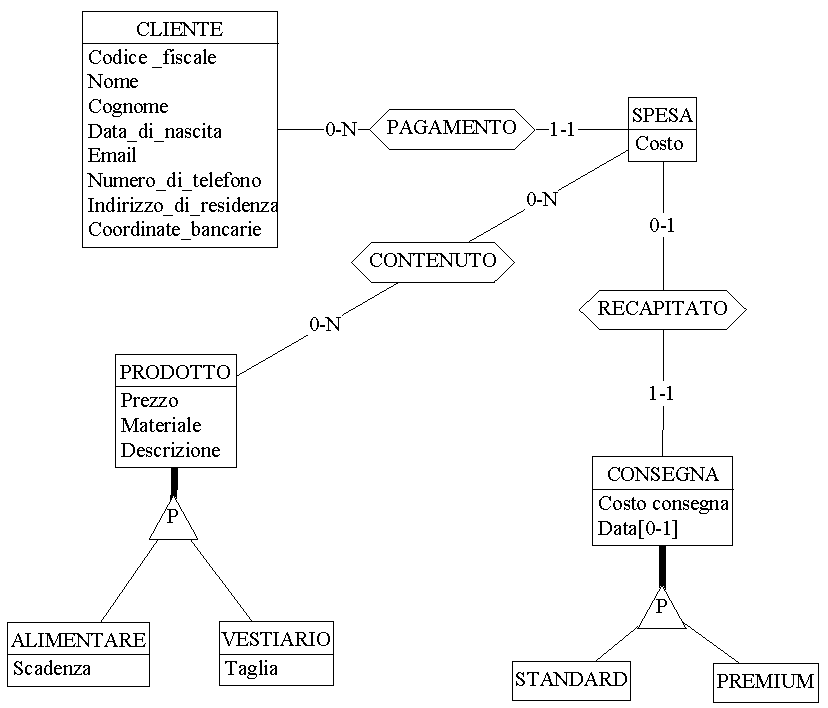
\includegraphics[width=\textwidth]{img/SchemaConcettuale-Clienti1.pdf}
	\caption{Schema scheletro per i Clienti}
\end{figure}
\subsection{Raffinamenti proposti}
L'entità Cliente è una estensione di un'entità generica Persona, che si decide di aggiungere allo schema. 
L'entità Prodotto non permette di mantenere uno storico dei diversi prezzi e delle diverse "versioni" dello stesso prodotto, come la taglia o la scadenza. 
Per questo si decide di creare un'entità Prodotto in Vendita che è il prodotto venduto al cliente, collegato a Prodotto via Commercializzato e si aggiungono al Prodotto in Vendita il prezzo e il periodo di validità del prezzo. 
Come identificatori per l'entità cliente si usa un codice univoco (per evitare l'omocodia del codice fiscale), per Spesa e Prodotto e Consegna si usa un codice univoco. Prodotto In Vendita usa come identificatore l'identificatore di Prodotto e la data di inizio di vendita.
\subsection{Schema concettuale parziale}
\begin{figure}[h]
	\centering{}
	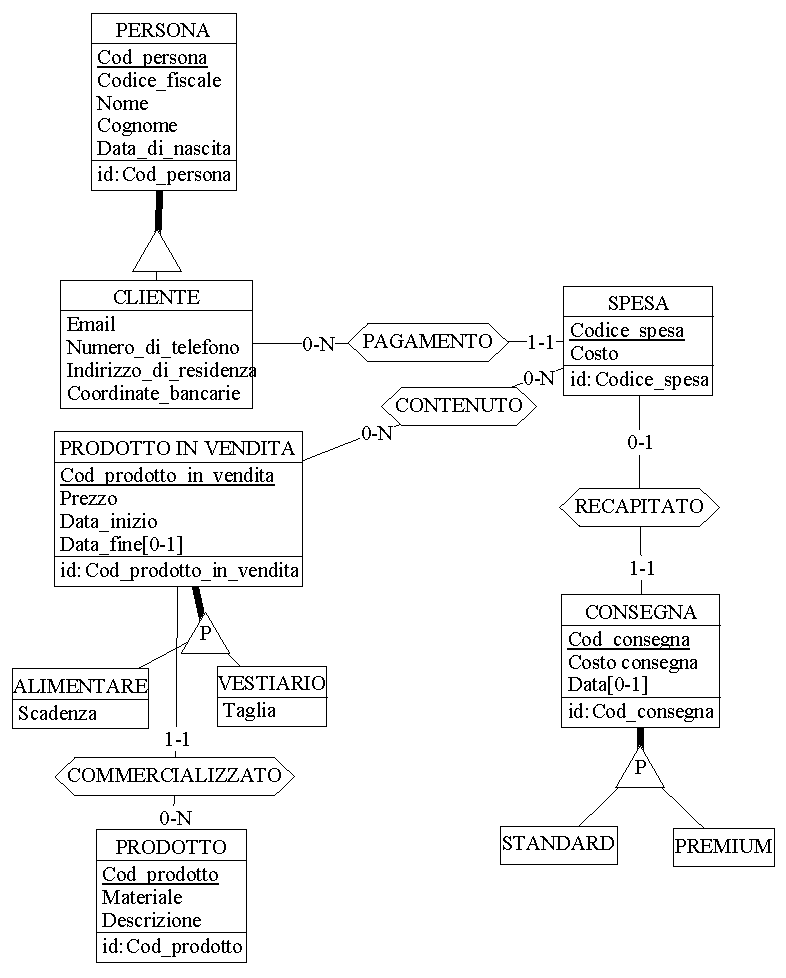
\includegraphics[width=\textwidth]{img/SchemaConcettuale-Clienti2.pdf}
	\caption{Schema scheletro per i Clienti, dopo le modifiche apportate}
\end{figure}
\section{Corrieri}
\subsection{Schema scheletro}
Dopo aver esaminato il dominio del problema per la parte dei corrieri, viene proposto il seguente schema scheletro.
\begin{figure}[h]
	\centering{}
	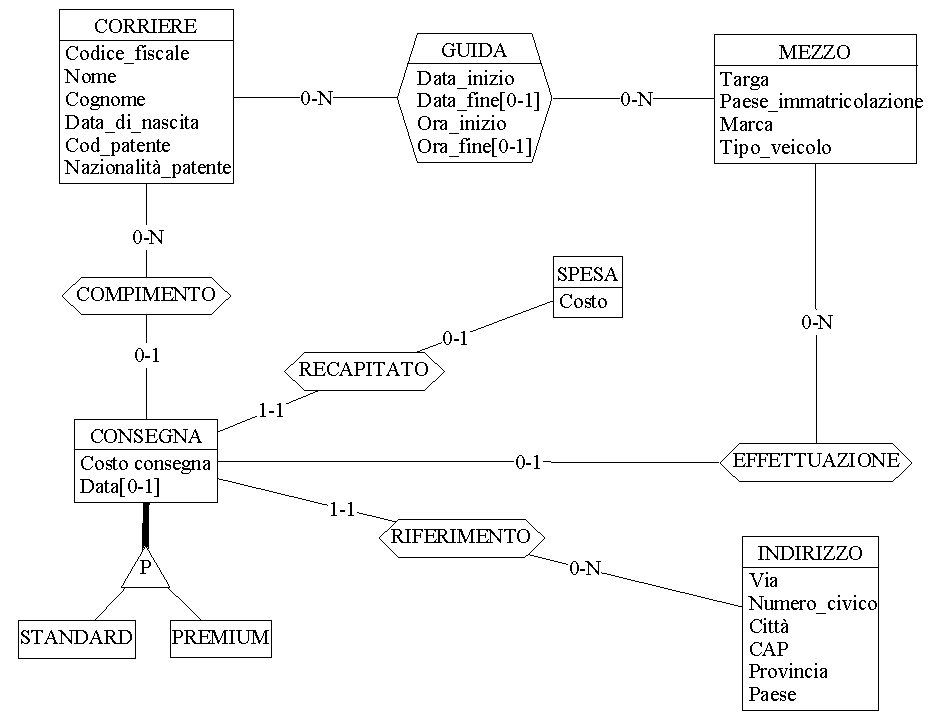
\includegraphics[width=\textwidth]{img/SchemaConcettuale-Corrieri1.pdf}
	\caption{Schema scheletro per i Corrieri}
\end{figure}
\subsection{Raffinamenti proposti}
L'entità Corriere è una estensione di un'entità generica Persona, che si decide di aggiungere allo schema. 
La relazione Guida non è corretta rappresentata come relazione perchè questo impedisce ad un corriere di guidare lo stesso mezzo più volte. 
Guida diventa una entità quindi, in relazione 1-1 con Corriere attraverso Conducente e attraverso Utilizzo per Mezzo, mentre le cardinalità dai lati delle entità rimangono 0-N. 
Come identificatori per Corriere si può usare il codice di persona oppure il codice della patente. 
Per Mezzo come identificatore uso la Targa, per Consegna,Spesa e Indirizzo un codice univoco. 
Gli identificatori di guida sono due i possibili, o l'identificatore di Corriere unito alla data ed ora oppure l'identificatore di Mezzo unito alla data ed ora. 
Un vincolo inespresso è il fatto che più guide dello stesso corriere possono avvenire contemporaneamente. 
\subsection{Schema concettuale parziale}
\begin{figure}[h]
	\centering{}
	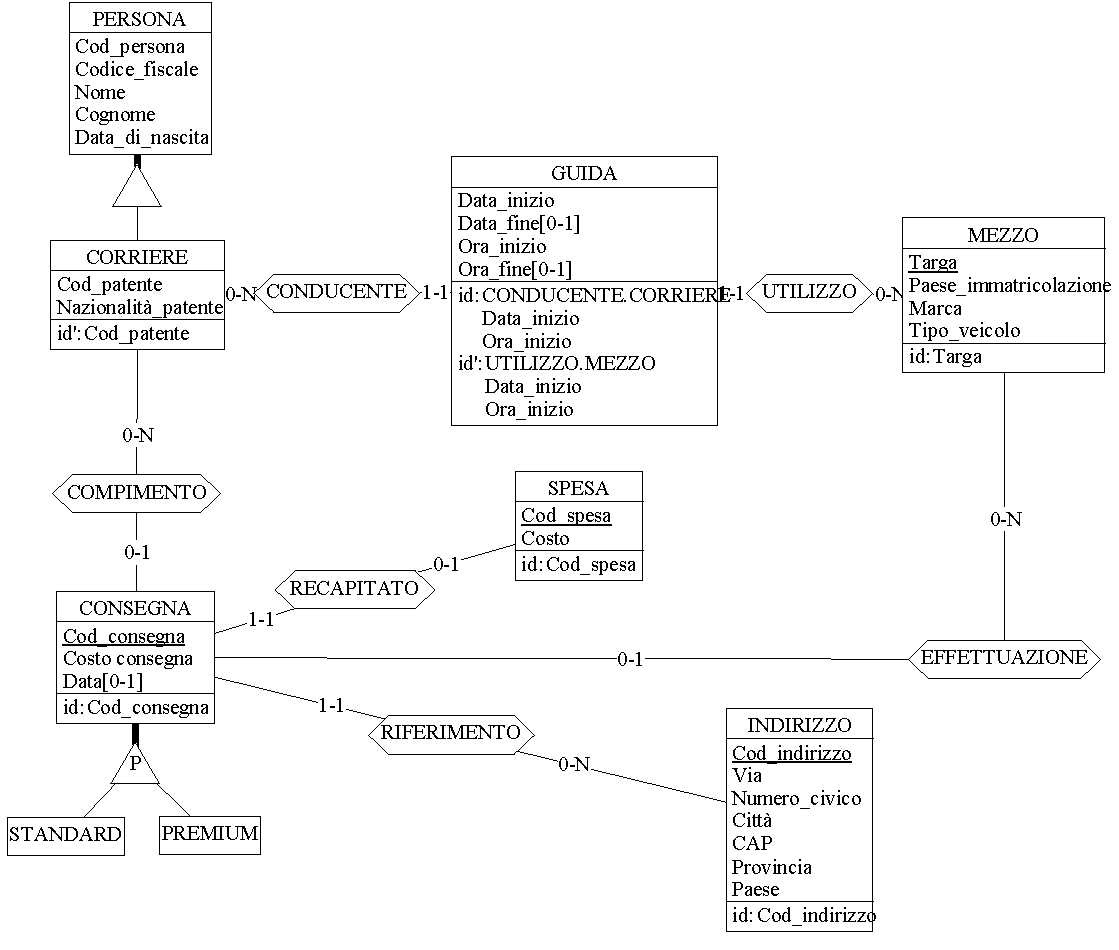
\includegraphics[width=\textwidth]{img/SchemaConcettuale-Corrieri2.pdf}
	\caption{Schema scheletro per i Corrieri, dopo le modifiche apportate}
\end{figure}
\section{Produttore}
\subsection{Schema scheletro}
Dopo aver esaminato il dominio del problema per la parte dei produttori, viene proposto il seguente schema scheletro.
\begin{figure}[h]
	\centering{}
	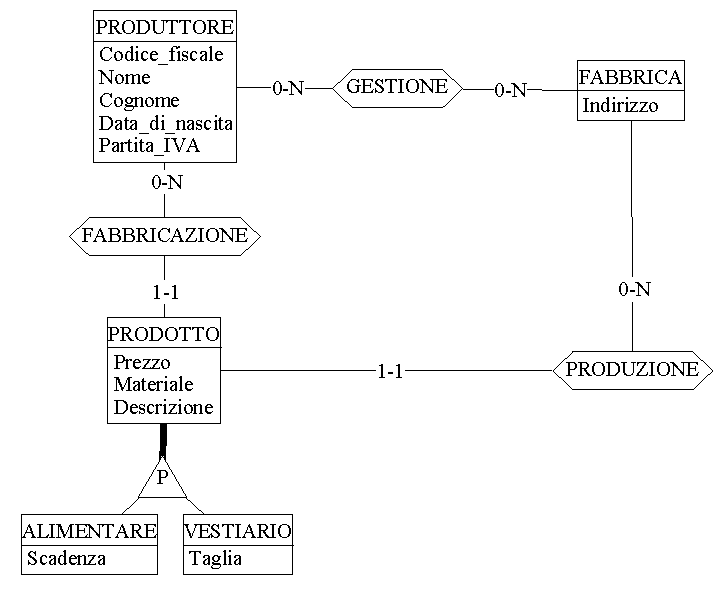
\includegraphics[width=\textwidth]{img/SchemaConcettuale-Produttori1.pdf}
	\caption{Schema scheletro per i Produttori}
\end{figure}
\subsection{Raffinamenti proposti}
Come per Corriere e Cliente, Produttore è estensione dell'entità generica Persona, che viene aggiunta. 
La relazione gestische tra Produttore e Fabbrica non è corretta, perchè non si riesce a mantenere uno storico dei diversi produttori di una fabbrica.
Perciò si decide di trasformarla in una entità, con attributi la data di inizio e la eventuale data di fine gestione della fabbrica. Viene collegata da relazioni 1-1 verso Produttore attraverso la relazione Gestione e con Amministrazione verso Fabbrica, e si mantiene 0-N nel verso opposto.
Per mantenere lo storico dei prezzi dei prodotti si crea un'entità Prodotto In Vendita, come nello schema Clienti.
Come identificatore di Produttore si usa quello di Persona, per Fabbrica e Prodotto si usa un codice. Prodotto in Vendita usa come identificatore quello importato da Prodotto più la data.
\subsection{Schema concettuale parziale}
\begin{figure}[h]
	\centering{}
	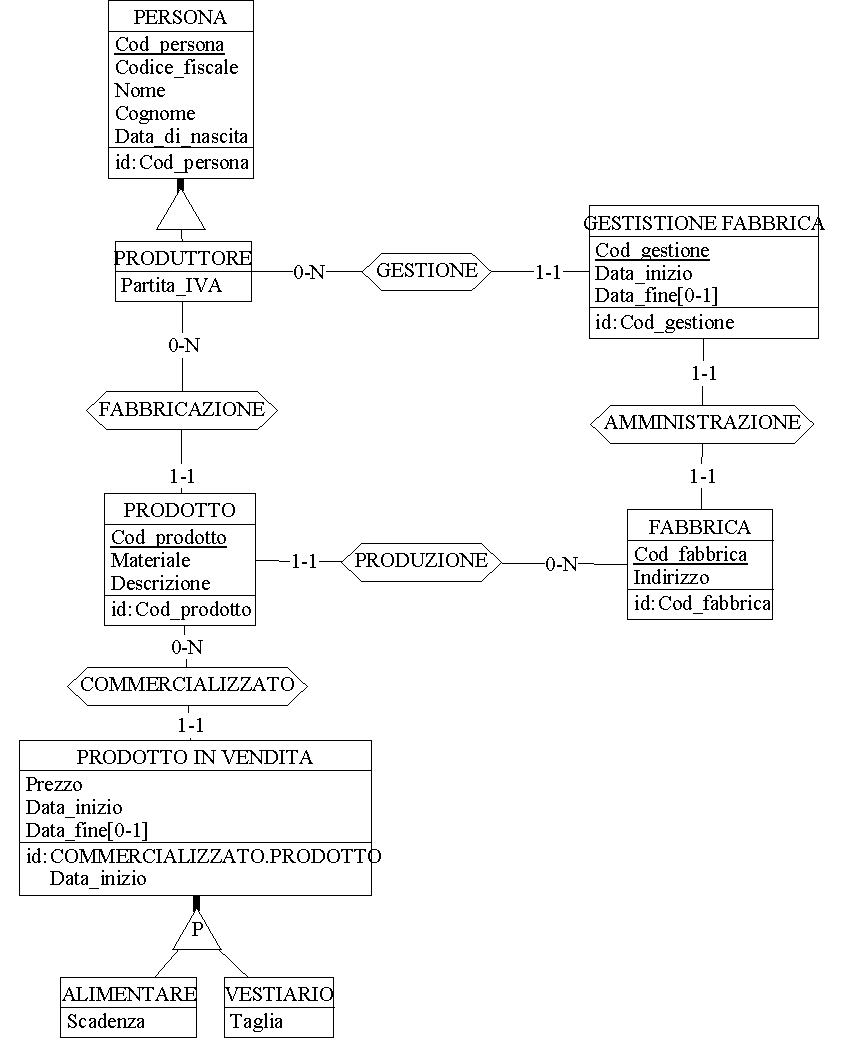
\includegraphics[width=\textwidth]{img/SchemaConcettuale-Produttori2.pdf}
	\caption{Schema scheletro per i Produttori, dopo le modifiche apportate}
\end{figure}
\section{Integrazione delle viste}
Nei seguenti schemi vengono mostrate solo le entità e relazioni che servono per unire le viste, per rendere migliore l'immagine. Lo schema finale completo è nella sezione successiva.
\subsection{Unione tra Corrieri e Clienti}
L'unione tra Corrieri e Clienti avviene in due entità. Sia Cliente che Corriere sono generalizzazioni di Persona, quindi vengono unite nella gerarchia totale ed esclusiva.
\begin{figure}[h]
	\centering{}
	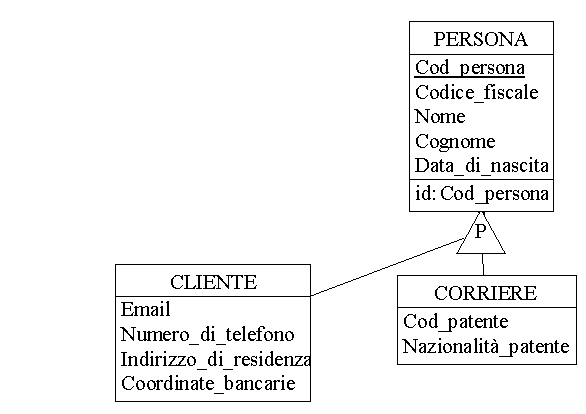
\includegraphics[width=\textwidth]{img/Unione-Clienti-Corrieri1.pdf}
	\caption{Unione di Corrieri e Clienti, via Persona}
\end{figure}
Un'altra unione degli schemi concettuali avviene in corrispondenza dell'entità Consegna, che è presente in entrambi gli schemi. 
\begin{figure}[h]
	\centering{}
	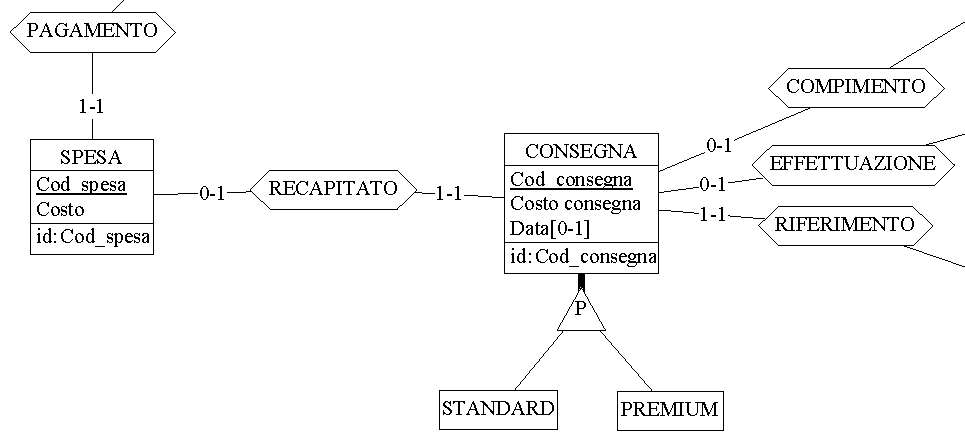
\includegraphics[width=\textwidth]{img/Unione-Clienti-Corrieri2.pdf}
	\caption{Unione di Corrieri e Clienti, via Consegna}
\end{figure}
\subsection{Unione tra Clienti e Produttori}

L'unione tra Produttori e Clienti avviene in due entità. Sia Cliente che Produttore sono generalizzazioni di Persona, quindi vengono unite nella gerarchia totale ed esclusiva. Nell'immagine compare anche Corrriere per l'unione degli schemi precedente.
\begin{figure}[h]
	\centering{}
	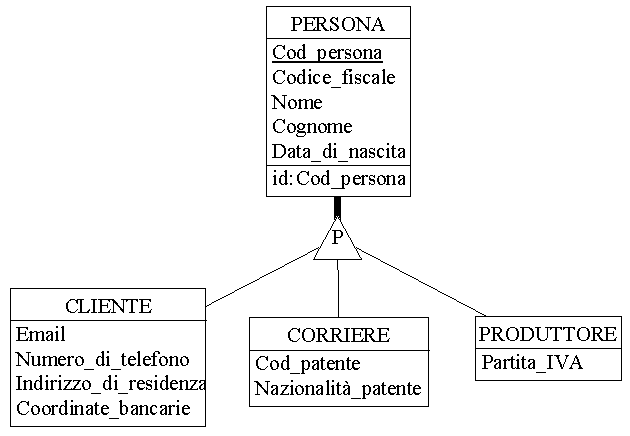
\includegraphics[width=\textwidth]{img/Unione-Clienti-Produttori1.pdf}
	\caption{Unione di Corrieri e Produttore, via Persona}
\end{figure}
Un'altra unione degli schemi concettuali avviene in corrispondenza dell'entità Prodotto e Prodotto in Vendita, che è presente in entrambi gli schemi. 
\begin{figure}[h]
	\centering{}
	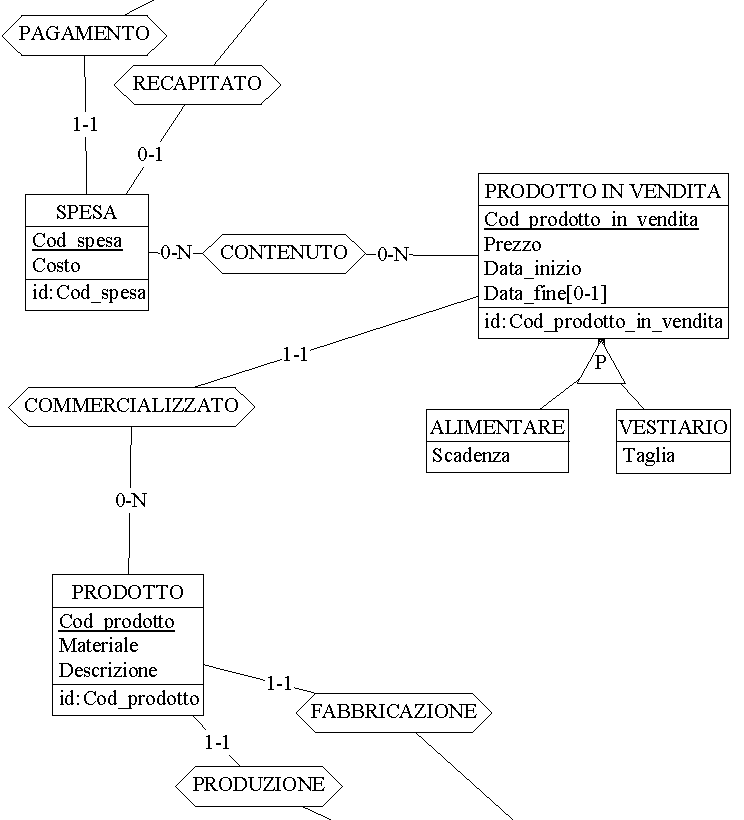
\includegraphics[width=\textwidth]{img/Unione-Clienti-Produttori2.pdf}
	\caption{Unione di Corrieri e Clienti, via Prodotto e Prodotto in Vendita}
\end{figure}

\section{Schema concettuale finale}
Lo schema concettuale finale, dopo l'integrazione delle viste:
\begin{figure}[h]
	\centering{}
	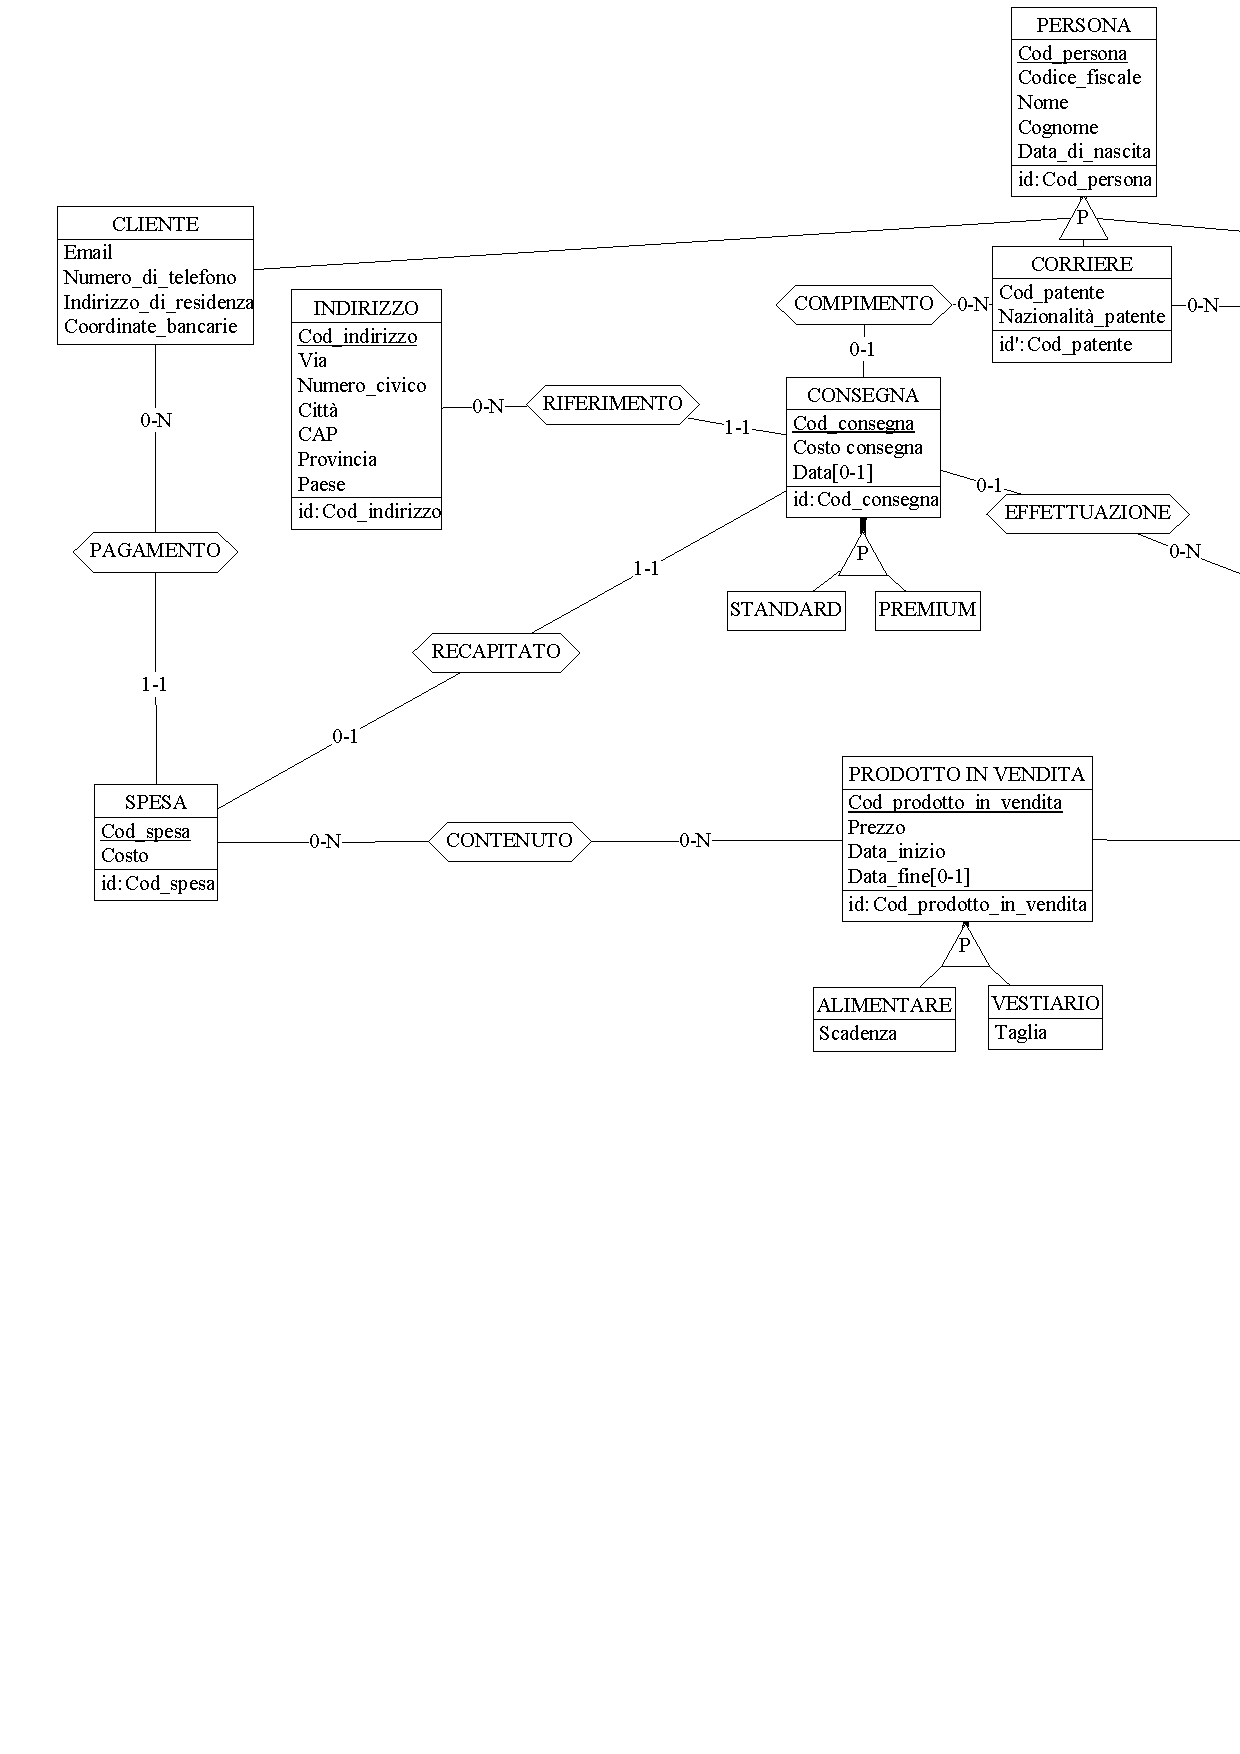
\includegraphics{img/SchemaConcettuale-fin1.pdf}
	\caption{Lo schema concettuale finale, prima pagina}
\end{figure}
\begin{figure}[h]
	\centering{}
	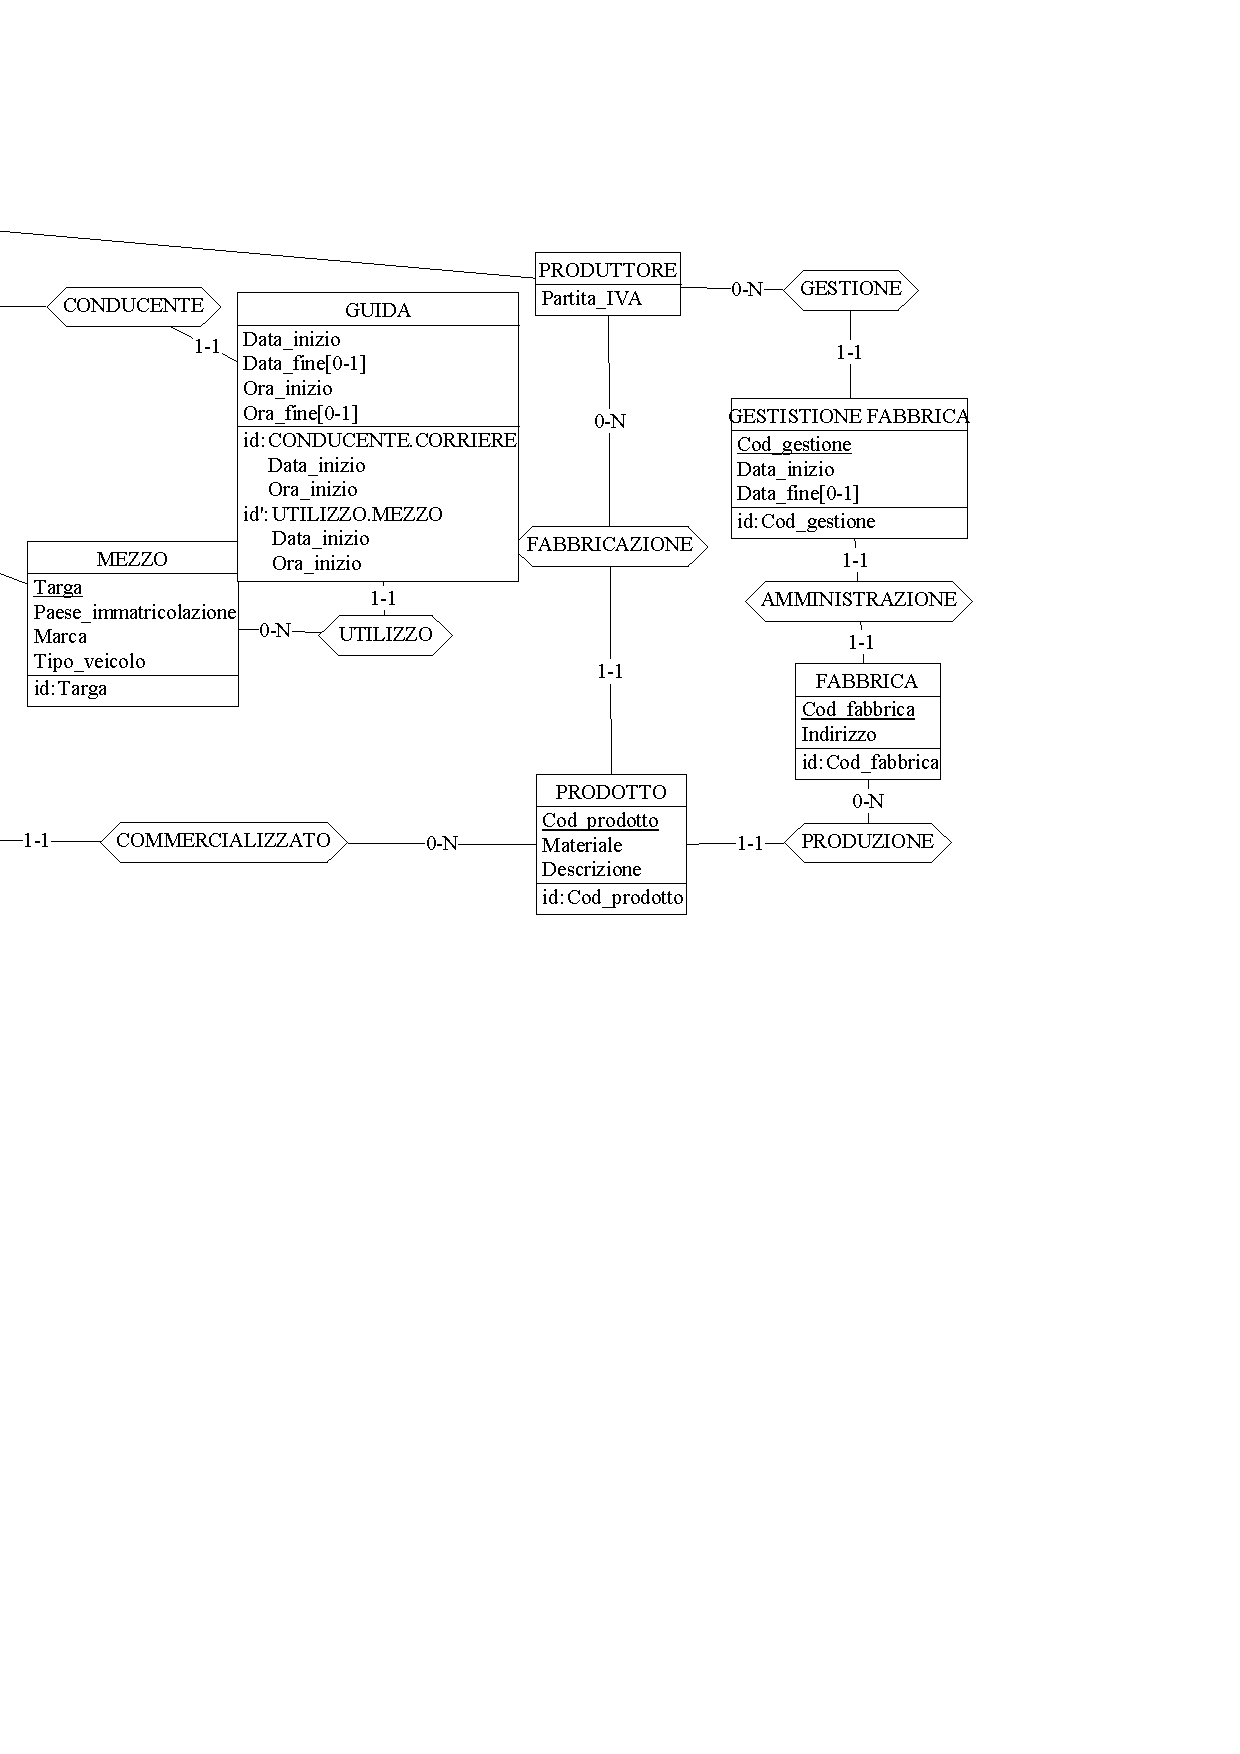
\includegraphics{img/SchemaConcettuale-fin2.pdf}
	\caption{Lo schema concettuale finale, seconda pagina}
\end{figure}

\chapter{Progettazione Logica}
\section{Stima del volume dei dati}
\begin{center}
    \begin{tabular}{ | c  c  c|} 
    \hline
    Concetto&Costrutto&Volume \\
    \hline
	\hline
    Cliente&E&0 \\
	Spesa&E&0 \\
	Pagamento&R&0 \\
	Prodotto in Vendita&E&0 \\
	%Alimentare/Vestiario?
	Contenuto&R&0 \\
	Prodotto&E&0 \\
	Storico Prezzi&R&0 \\
	Fabbrica&E&0 \\
	Creato in&R&0 \\
	Gestione Fabbrica&E&0 \\
	Amministrata&R&0 \\
	Produttore&E&0\\
	Gestisce&R&0 \\
	Produce&R&0\\
	Corriere&E&0\\
	Guida&E&0\\
	Conduce&R&0\\
	Mezzo&E&0\\
	Utilizzato&R&0\\
	Consegna&E&0\\
	%o i figli?
	Effettua&R&0\\
	Attraverso&R&0\\
	Indirizzo&E&0\\
	Riferisce&R&0\\
	Viene Recapitata&R&0\\
    \hline
    \end{tabular}
\end{center}
\section{Descrizione delle operazioni principali e stima della loro frequenza}
\begin{center}
    \begin{tabular}{ | c | c | c |} 
    \hline
    Codice&Operazione&Frequenza\\
    \hline
	1&Inserire un nuovo cliente&1000 al giorno\\
	\hline
	2&Cambiare il prezzo ad un prodotto esistente&100 al giorno\\
	\hline
	3&Creare una nuova guida ad un corriere ed un mezzo esistenti&200 al giorno\\
	\hline
	4&Leggere il prezzo medio di un prodotto&10 al giorno\\
	\hline
	5&Leggere quale corriere ha consegnato una data spesa&100 al giorno\\
	\hline
	6&Trovare il produttore di un dato prodotto&1000 al giorno\\
	\hline
	7&Creare una nuova spesa&100 al giorno\\
	\hline
	8&Leggere l'indirizzo associato ad una consegna&2000 al giorno\\
	\hline
	9&Cercare un prodotto di una taglia specifica&100 al giorno\\
	\hline 
	10&Cercare tutte le consegne di un corriere&20 al giorno\\
	\hline
	11&Ricavare l'ultima consegna ad un cliente&100 al giorno\\
	\hline
	12&Cambiare gestione ad una fabbrica&1 al giorno\\
	\hline
	13&Inserire un nuovo mezzo&2 al giorno\\
	\hline
    \end{tabular}
\end{center}
\section{Schemi di navigazione e tabelle degli accessi}
Sono riportate in seguito gli accessi necessarie per eseguire le operazioni riportate. 
Gli schemi di navigazione sono presenti solo per operazioni non banali. Per calcolare i costi si considera un accesso in scrittura come doppio rispetto a uno in lettura.
\section{Raffinamento dello schema}
eliminazione di identificatori esterni, attributi composti e gerarchie, scelta delle chiavi
subsection per ognuno di questi lavori
\section{Analisi delle ridondanze}
Ridondanze, conti
\section{Traduzione di entità e associazioni in relazioni}
Traduzione ER
\section{Schema relazionale finale}
Schema finale
\section{Traduzione delle operazioni in query SQL}
delle operazioni

\chapter{Progettazione dell'applicazione}
\section{Descrizione dell'architettura dell'applicazione}
Java, operazioni banali (inserimento, ecc)
realizzata con obbligo di inserire alcuni screenshot dell'interfaccia utente
diverse schermate (utente, corriere, ecc)
tabella operazione originale -> metodo/classe
\end{document}